% Modified from AAAS Science LATEX template
% Use only LaTeX2e, calling the article.cls class and 12-point type.

\documentclass[11pt, a4paper, oneside]{article}
\usepackage{helvet}
\renewcommand{\familydefault}{\sfdefault}

\usepackage{graphicx}

\usepackage{caption}
\captionsetup{font=small}
\usepackage{url}

\usepackage{scicite}

% Page setup

\topmargin 0.0cm
\oddsidemargin 0.2cm
\textwidth 16cm
\textheight 21cm
\footskip 1.0cm

\usepackage[legalpaper, portrait, margin=0.5in]{geometry}

% Abstract environment
\newenvironment{sciabstract}{%
\begin{quote} \bf}
{\end{quote}}

% Paper title
\title{
XPRESSyourself: Automating and Democratizing High-Throughput Sequencing
}

% Author info
\author{
Tentative author list/order:
Jordan A. Berg,$^{1}$ Jonathan R. Belyeu,$^{2}$ Jeffrey T. Morgan,$^{1}$ Alex J. Bott,$^{1}$ \\
Yeyun Ouyang,$^{1}$ Jason Gertz,$^{3}$ Aaron R. Quinlan,$^{2,4,5}$ Michael T. Howard,$^{2}$ Jared P. Rutter$^{1,6\ast}$\\
\\
\normalsize{$^{1}$Department of Biochemistry, University of Utah, Salt Lake City, UT, USA, 84112}\\
\normalsize{$^{2}$Department of Human Genetics, University of Utah, Salt Lake City, UT, USA, 84112}\\
\normalsize{$^{3}$Department of Oncological Sciences, University of Utah, Salt Lake City, UT, USA, 84112}\\
\normalsize{$^{4}$USTAR Center for Genetic Discovery, University of Utah, Salt Lake City, UT, USA, 84112}\\
\normalsize{$^{5}$Department of Biomedical Informatics, University of Utah, Salt Lake City, UT, USA, 84112}\\
\normalsize{$^{6}$Howard Hughes Medical Institute, University of Utah, Salt Lake City, UT, USA, 84112}\\
\\
\normalsize{$^\ast$To whom correspondence should be addressed; E-mail: rutter@biochem.utah.edu.}
}

% Include the date command, but leave its argument blank.
\date{}

%%%%%%%%%%%%%%%%% END OF PREAMBLE %%%%%%%%%%%%%%%%


% Initialize use of code blocks with syntax highlighting

\usepackage{listings}
\usepackage{color}

\definecolor{dkgreen}{rgb}{0,0.6,0}
\definecolor{gray}{rgb}{0.5,0.5,0.5}
\definecolor{mauve}{rgb}{0.58,0,0.82}

\lstset{frame=tb,
  language=Java,
  aboveskip=3mm,
  belowskip=3mm,
  showstringspaces=false,
  columns=flexible,
  basicstyle={\small\ttfamily},
  numbers=none,
  numberstyle=\tiny\color{gray},
  keywordstyle=\color{blue},
  commentstyle=\color{dkgreen},
  stringstyle=\color{mauve},
  breaklines=true,
  breakatwhitespace=true,
  tabsize=3
}


\begin{document}

% Double-space the manuscript.
\baselineskip24pt

% Make the title.
\maketitle



% Place your abstract within the special {sciabstract} environment.
\begin{sciabstract}
With the advent of high-throughput sequencing platforms, expression profiling is becoming common-place in medical research. However, for the general user, a computational overhead often exists. The XPRESSyourself suite aims to reduce these barriers to entry for those with limited or advanced computational experience alike and create a series of tools aimed at standardizing and increasing throughput of data processing and analysis. The XPRESSyourself suite is currently broken down into two software packages. The first, XPRESSpipe, automates the pre-processing, alignment, quantification, normalization, and quality control of single-end, paired-end RNAseq, and ribosome profiling sequence data. The second, XPRESStools, is a Python toolkit for expression data analysis, compatible with private or RNAseq datasets. This software suite is designed to be easily be modified, and additional packages can be included for processing of other data types in the future, such as CHIPseq or genome alignment. In addition, this package offers several new tools useful in processing RNA-seq data, specifically for ribosome profiling. We validated the performance of this suite by processing and analyzing pubilcly available datasets and comparing the output with published results. Use of this pipeline will close gaps in the stardardization of RNA-seq processing and democratize the RNA-seq bioinformatic experience.
% To demonstrate the capability of this software package, we analyzed a publicly available ribosome profiling dataset and identified new metabolic insights into the ER-stress response.
\newline\\
\normalfont XPRESSyourself is freely available on GitHub: https://github.com/XPRESSyourself\\
\end{sciabstract}


\section{Introduction}

High-throughput profiling of gene expression data has revolutionized biomedical, industrial, and basic science research. Within the last two decades, RNA-seq has found itself the forerunner technology for high quality gene expression profiling, as it can measure relative transcript abundance, differential splice variants, sequence polymorphisms, and more \cite{byron_nrg}. This technology has also been adopted to create technologies such as single-cell RNA-seq, capable of assaying the transcriptional profile cell by cell; and ribosome profiling, which measures ribosome occupancy and translation efficiency \cite{ingolia_science}.

While vast strides have been made to these technologies, various bottlenecks still exist. For example, while more and more researchers are becoming accustomed to to the field of bioinformatics and computational biology, learning the intricracies of the different tools used in processing RNA-seq data can be inhibitory if users are not aware of the proper tools to use or use outdated software \cite{costello_npjsba, funari_science}. Even for the experienced user, developing robust, automated pipelines that process and check datasets can be laborious and introduce variability to data processing.

While several computational pipelines for sequencing have emerged intending to tackle various aspects of these bottlenecks, many suffer from usability issues, are not easily modifiable, or sacrifice quality for speed. Additionally, few if any offer a thorough set of integrated tools for handling common quality control issues or reference creation. For example, a common bias in ribosome profiling libraries is a 5' transcript pile-up \cite{gerashchenko_nar, artieri_gr, hussman_plosg}. It is recommended that this region of each transcript not be quantified when processing ribosome profiling libraries; however, currently no tools exist to aid the general user in doing so \cite{ingolia_meth, weinberg_reports}.

In response to the issues surrounding the automation and democratization of sequencing technology, we created the XPRESSyourself bioinformatics suite for processing and analyzing high-throughput expression data. In creating this tool, we focused on usefulness, usability, reliability, efficiency, and flexibility \cite{taschuk_ploscb}. With the XPRESSyourself package XPRESSpipe, the user is provided with a complete suite of software to handle pre-processing, aligning, and quantifying reads, performing quality control via various meta-analyses of pre- and post-processed reads. We also provide access to key quality control measures useful for assessing RNA-seq and ribosome profiling experiments. These include read length distributions to ensure correct sequencing library read sizes and a periodicity sub-module that tracks the P-site of ribosome footprints to assess effective capture of the ribosome's characteristic 1 codon step. These measures are particular helpful for ribosome profiling experiments. XPRESSpipe also includes a metagene analysis sub-module that shows the distribution of all aligned reads across a representative transcript a library and a library complexity visualization sub-module to ensure minimalization of PCR duplicates. Additionally, housed within the XPRESSyourself XPRESStools package, tools are provided to perform the bulk of sequence analysis and generation of figures for publication.

\section{Materials and Methods}

\subsection{XPRESSpipe}
XPRESSpipe pipelines for single-end RNA-seq, paired-end RNA-seq, and ribosome profiling offer a handful of tunable parameters to the user, while keeping most parameters hidden to maintain The Cancer Genome Atlas (TCGA) (https://www.cancer.gov/tcga) alignment standards and ensure standardization of alignment. In the future it is feasible that additional tunable parameters will be added. For the purposes of this manuscript, we will focus on ribosome profiling examples, while the majority of statements are applicable to single- and paired-end RNA-seq. More details can be found in the documentation (https://xpresspipe.readthedocs.io/en/latest/). Table \ref{Tab:xpresspipe} outlines these parameters.

\captionof{table}{Summary of XPRESSpipe pipeline arguments.\label{Tab:xpresspipe}}
\begin{tabular}{p{5cm}p{13cm}}
 \textbf{Arguments} & \textbf{Description} \\
 \hline
 \textbf{Required} & \\
 \hline
 \texttt{-i, --input} & Path to input directory \\
 \hline
 \texttt{-o, --output} & Path to output directory \\
 \hline
 \texttt{-r, --reference} & Path to parent organism reference directory \\
 \hline
 \texttt{-g, --gtf} & Path and file name to GTF used for alignment quantification \\
 \hline
 \texttt{-e, --experiment} & Experiment name \\
 \hline
 \textbf{Optional} & \\
 \hline
 \texttt{-a, --adaptors} & Specify adaptor as string (only one allowed) -- if ``None" is provided, software will attempt to auto-detect adaptors -- if ``POLYX" is provided as a single string in the list, polyX adaptors will be trimmed \\
 \hline
 \texttt{-q, --quality} & PHRED read quality threshold (default: 28) \\
 \hline
 \texttt{--min\_length} & Minimum read length threshold to keep for reads (default: 18) \\
 \hline
 \texttt{--output\_bed} & Include option to output BED files for each aligned file \\
 \hline
 \texttt{--output\_bigwig} & Include flag to output bigwig files for each aligned file \\
 \hline
 \texttt{--method} & Normalization method to perform (options: ``RPM", ``TPM", ``RPKM", ``FPKM", ``LOG") \\
 \hline
 \texttt{--batch} & Include path and filename of dataframe with batch normalization parameters \\
 \hline
 \texttt{--sjdbOverhang} & Sequencing platform read-length for constructing splice-aware reference previously (see documentation for more information) \\
 \hline
 \texttt{-m, --max\_processors} & Number of max processors to use for tasks (default: No limit) \\
\end{tabular}
\newline

\subsubsection{Installation}
XPRESSpipe can be compiled from source (https://github.com/XPRESSyourself/XPRESSpipe) or a version-controlled Docker image (https://www.docker.com/) can be loaded using the following commands:
\newline

% Install XPRESSpipe code block
\begin{lstlisting}[language=bash, caption=curateReference example]
$ docker image pull jordanberg/xpresspipe:latest
\end{lstlisting}

% Software dependencies table
\captionof{table}{Summary of dependency software, accession location, and purpose in the XPRESSpipe package.\label{Tab:packages}}
\begin{tabular}{p{2.4cm}p{7.5cm}p{3cm}}
 \textbf{Package} & \textbf{Purpose} & \textbf{Reference} \\
 \hline
 fastp & Read pre-processing & \cite{fastp} \\
 \hline
 STAR & Reference curation and read alignment & \cite{star} \\
 \hline
 samtools & Alignment file manipulation & \cite{samtools} \\
 \hline
 bedtools & Alignment file manipulation & \cite{bedtools} \\
 \hline
 deeptools & Alignment file manipulation & \cite{deeptools} \\
 \hline
 htseq & Read quantification & \cite{htseq} \\
 \hline
 fastqc & Quality Control & \cite{fastqc} \\
 \hline
 multiqc & Quality Control & \cite{multiqc} \\
 \hline
 DESeq2 & Perform differential expression analysis & \cite{deseq2} \\
 \hline
 dupRadar & Measure library complexity & \cite{dupradar} \\
 \hline
 pandas & Data manipulation & \cite{pandas} \\
 \hline
 numpy & Data manipulation & \cite{numpy1, numpy2} \\
 \hline
 scipy & Data manipulation & \cite{scipy} \\
 \hline
 matplotlib & Plotting & \cite{matplotlib} \\
 \hline
 xpresstools & Normalization and matrix manipulation & This paper \\
\end{tabular}
\newline

XPRESSpipe is built upon several pre-established software packages, listed in Table \ref{Tab:packages}. These dependencies are included in any Docker images for XPRESSpipe; however, if installing manually, these packages will need to be installed by the user.

\subsubsection{Inputs}
While inputs will vary sub-module to sub-module, and further information can be found in the documentation (https://xpresspipe.readthedocs.io/en/latest/) or by entering \texttt{xpresspipe \textless sub-module name\textgreater \ --help}, a few points of guidance are important to consider.

\begin{itemize}
\item Single-end reads should end in \texttt{.fa}, \texttt{.fasta}, or \texttt{.txt}
\item Paired-end reads should end in \texttt{.read1/2.fa} or \texttt{.r1/2.fa}, where \texttt{.fa} could also be \texttt{.fasta} or \texttt{.txt}
\item The transcriptome reference file should be a valid GTF file and should be named \texttt{transcripts.gtf}
\item If specifying a group of fasta files to use for alignment or reference curation, the directory containing these files cannot contain any other files ending in \texttt{.txt} or \texttt{.fa}
\end{itemize}

Other sub-modules that handle a point in the middle of sequence processing need to be of appropriate file type, explained more in the help menu or documentation.

\subsubsection{Reference Curation}
One of the first preparatory steps of RNAseq alignment is curating a reference for the alignment software to map reads. For the purposes of the current version of XPRESSpipe, a STAR \cite{star} reference should be created. An Ensembl-formatted (https://ensembl.org) GTF should also be placed in the reference directory and be named \texttt{transcripts.gtf}. Additional modifications are recommended to this file, which can be performed using the \texttt{modifyGTF} sub-module. Modifications include removing all genes not annotated as protein-coding and/or retaining only the longest transcript for each gene. For the purposes of ribosome profiling, where 5' and 3' transcript biases are frequent \cite{ingolia_meth, weinberg_reports}, the 5' and 3' ends of each gene record can be trimmed using the same function. While each of these steps are available as stand-alone sub-modules, all reference files used by XPRESSpipe, including STAR files and modified transcriptome files can be created by running the \texttt{curateReference} command. An example is shown below for creating a ribosome profiling-ready reference XPRESSpipe directory. The following assumes one is avoiding mapping to the first 45 nucleotides and last 15 nucleotides of the longest transcript for each gene, will only quantify to protein coding regions, and is tailored for mapping 50-bp single-end RNA-seq reads. As this can be a time-consuming process, we will leave the \texttt{--max\_processors} argument as default in order to utilize all cores available to the computing unit.
\newline
\begin{lstlisting}[language=bash, caption=curateReference example]
$ xpresspipe curateReference -o /path/to/output/location/ \
                                -f /path/to/fasta/genome/files/ \
                                -g /path/transcripts.gtf \
                                --protein_coding \
                                --longest_transcript \
                                --truncate \
                                --truncate_5prime 45 \
                                --truncate_3prime 15 \
                                --sjdbOverhang 49 \
                                --max_processors None
\end{lstlisting}

\subsubsection{Read Processing}
While all intermediate steps of the pipelines can be run singly, we will describe the outline of the software in the context of the pipelines. Pipelines and individual sub-modules are capable of being run in a parallel manner for each input file, thus accelerating the overall process. Descriptions of the options can be found in Table \ref{Tab:xpresspipe}.

\begin{enumerate}
  \item \textbf{Trim}: First, reads need to be cleaned of artifacts for the library preparation and sequencing process. These include adaptors, unique molecular identifier (UMI) sequences, and base calls with low confidence. By doing so, non-native sequences are removed and reads can align properly to the reference sequence. XPRESSpipe uses fastp, a faster, more accurate trimming package that has improved alignable read output \cite{fastp}. Adaptor sequence, base quality, and read length are all adjustable parameters available to the user.
  \item \textbf{Align}: After trimming, reads are then aligned to a reference genome. XPRESSpipe uses STAR, which, while taking a memory intensive approach, is fast and one of the most best performing sequence alignment software packages currently available \cite{star, baruzzo_natmeth}. XPRESSpipe performs a two-pass alignment of reads wherein first splice junctions are mapped and built into the reference; and second, reads are mapped accounting for these junctions to improve mappability over these regions. A sorted-by-coordinate and indexed BAM file is output and only unique alignments pass on to the next steps. PCR duplicates are detected and marked or removed for downstream processing. Optionally, bed and bigwig files can also be output.
  \item \textbf{Count}: XPRESSpipe quantifies read alignments for each de-duplicated input file using htseq-count \cite{htseq}. If a modified GTF was provided as input, it is used here to avoid potential pitfalls with read quanitification (i.e. a read being counted as a multi-mapper when belonging to multiple transcripts for the same gene). By default, htseq behavior conforms to TCGA standards by being strand agnostic, mapping assuming reads were sorted by name, and by using the \texttt{intersection-nonempty} method for handling reads overlapping multiple genes.
  \item \textbf{Normalize}: Methods for count normalization are available within XPRESSpipe. For normalizations involving transcript length, the appropriate GTF (transcripts-only recommended) must be provided. For samples sequenced on different chips, prepared by different individuals, or on different days, the \texttt{--batch} argument should be provided along with the appropriate metadata matrix. Sample normalization methods available include reads-per-million (RPM), Reads-per-kilobase-million (RPKM) or Fragments-per-kilobase-million (FPKM), and transcripts per million (TPM) normalizatin, as outlined in Equations 1-4 \cite{evans_briefbio}.

  \begin{equation}
    RPM = \frac{(\#\ number\ reads\ per\ gene)\ \cdot\ 1e6}{(\#\ mapped\ reads\ per\ sample)}
  \end{equation}
  \begin{equation}
    RPKM = \frac{(\#\ number\ reads\ per\ gene)\ \cdot\ 1e6\ \cdot\ 1e3}{((\#\ mapped\ reads\ per\ sample)\ \cdot\ (gene\ length\ (bp))}
  \end{equation}
  \begin{equation}
    FPKM = \frac{(\#\ number\ fragments\ per\ gene)\ \cdot\ 1e6\ \cdot\ 1e3}{(\#\ mapped\ fragments\ per\ sample)\ \cdot\ (gene\ length\ (bp))}
  \end{equation}
  \begin{equation}
    TPM = \frac{(\#\ number\ fragments\ per\ gene)\ \cdot\ 1e3\ \cdot\ 1e6}{(gene\ length\ (bp))\ \cdot\ (\#\ mapped\ fragments\ per\ sample)}
  \end{equation}

  \item \textbf{Quality Control}:
  It is important to perform quality control of sequencing samples to ensure the interpreted results are reliable. XPRESSpipe performs a variety of quality control measures. For each analysis type, high-resolution, publication quality summary plots are output for all samples in a given experiment.

    \begin{itemize}
      \item \textbf{Read Length Distribution}: Per sample, the lengths of all reads are analyzed by FastQC \cite{fastqc}. By assessing the read distribution of each sample, the user can ensure the expected read size was sequenced. This is particularly helpful for ribosome profiling experiments as insertion of the requisite 21-30 nt ribosome footprints into the sequencing library was successful.

      \item \textbf{Library Complexity}: Analyzing library complexity is an effective methods for analyzing the robustness of a sequencing experiment of capturing various mRNA species. As the majority of RNA-seq preparation methods involve a PCR step, at times certain fragments are favored and over-replicated in contrast to others. By plotting the number of PCR replicates versus expression level, one can determine how successful the library preparation was at reducing these biases. The analysis is performed using the PCR duplicate-tagged BAM files output by XPRESSpipe for each sample by dupRadar \cite{dupradar}. Duplicate tagging is performed by samtools \cite{samtools}.

      \item \textbf{Metagene Estimation Profile}: In order to identify any general 5' or 3' biases in captured transcripts, a metagene profile can be created for each sample. This is performed by determining the meta-genomic coordinate \textit{M} for each aligned read, where \textit{L} is the leftmost coordinate of the mapped read and \textit{r} is the length of the mapped read. \textit{S} denotes the start coordinate for the transcript and \textit{l} is the cumulative length of all exons for the given transcript. The subscripted \textit{e} indicates the coordinate is relative to exon space, where intron space is not counting in the coordinate relative to the start of the transcript. Required inputs are an indexed bam file and an unmodified GTF reference file. For each mapped coordinate, the metagene position is calculated as:
      \begin{equation}
      \textit{M} = \frac{|(L\textsubscript{e}\ +\ \frac{1}{2}r)\ -\ S|\ \cdot\ 100}{\textit{l\textsubscript{e}}}
      \end{equation}

      In the case where a mapped coordinate falls within multiple genes, a penalty is assigned as:
      \begin{equation}
        \textit{c} = \frac{1}{\textit{n}}
      \end{equation}
      Where \textit{c} is the count score for a given meta-position and \textit{n} is the number of different transcripts a given coordinate mapped. To be counted or factored into the penalty, the meta-position coordinate must fall within exon space.

      \item \textbf{Codon Phasing/Periodicity Estimation Profile}: In ribosome profiling, a useful measure of a successful experiment comes by investigating the codon phasing of ribosome footprints \cite{}. To do so, the P-site is calculated for each mapped ribosome footprint by taking the genomic coordinate 16 nucleotides upstream of the 3' end of each transcript and measuring the distance in nucleotides along exon space to the start of the transcript \cite{}. \textit{p} is the distance from the start, \textit{L} is the leftmost coordinate of the mapped read, \textit{r} is the length of the mapped read, and \textit{S} denotes the start coordinate for the transcript. The superscript signs associated with \textit{p} indicate strandedness and the subscript \textit{e} indicates the coordinate is relative to exon space. The same inputs are required as for the \texttt{metagene} sub-module, and the penalty is calculated in the same manner.
      \begin{equation}
        \textit{p}\textsuperscript{+} = (\textit{L}\textsubscript{e}\ +\ \textit{r} - 16)\ -\ \textit{S}
      \end{equation}
      \begin{equation}
        \textit{p}\textsuperscript{-} = \textit{S}\ -\ (\textit{L}\textsubscript{e}\ +\ 16)
      \end{equation}

    \end{itemize}
\end{enumerate}


\subsubsection{Outputs}
While outputs will vary sub-module to sub-module, generally, the user will specify a parent output directory and necessary sub-directories will be created based on the step in the pipeline. Further information can be found in the documentation (https://xpresspipe.readthedocs.io/en/latest/) or by entering \texttt{xpresspipe \textless sub-module name\textgreater \ --help}. Figure \ref{fig:outputs} provides an example of the output file scheme for XPRESSpipe.

\begin{figure}
\centering
  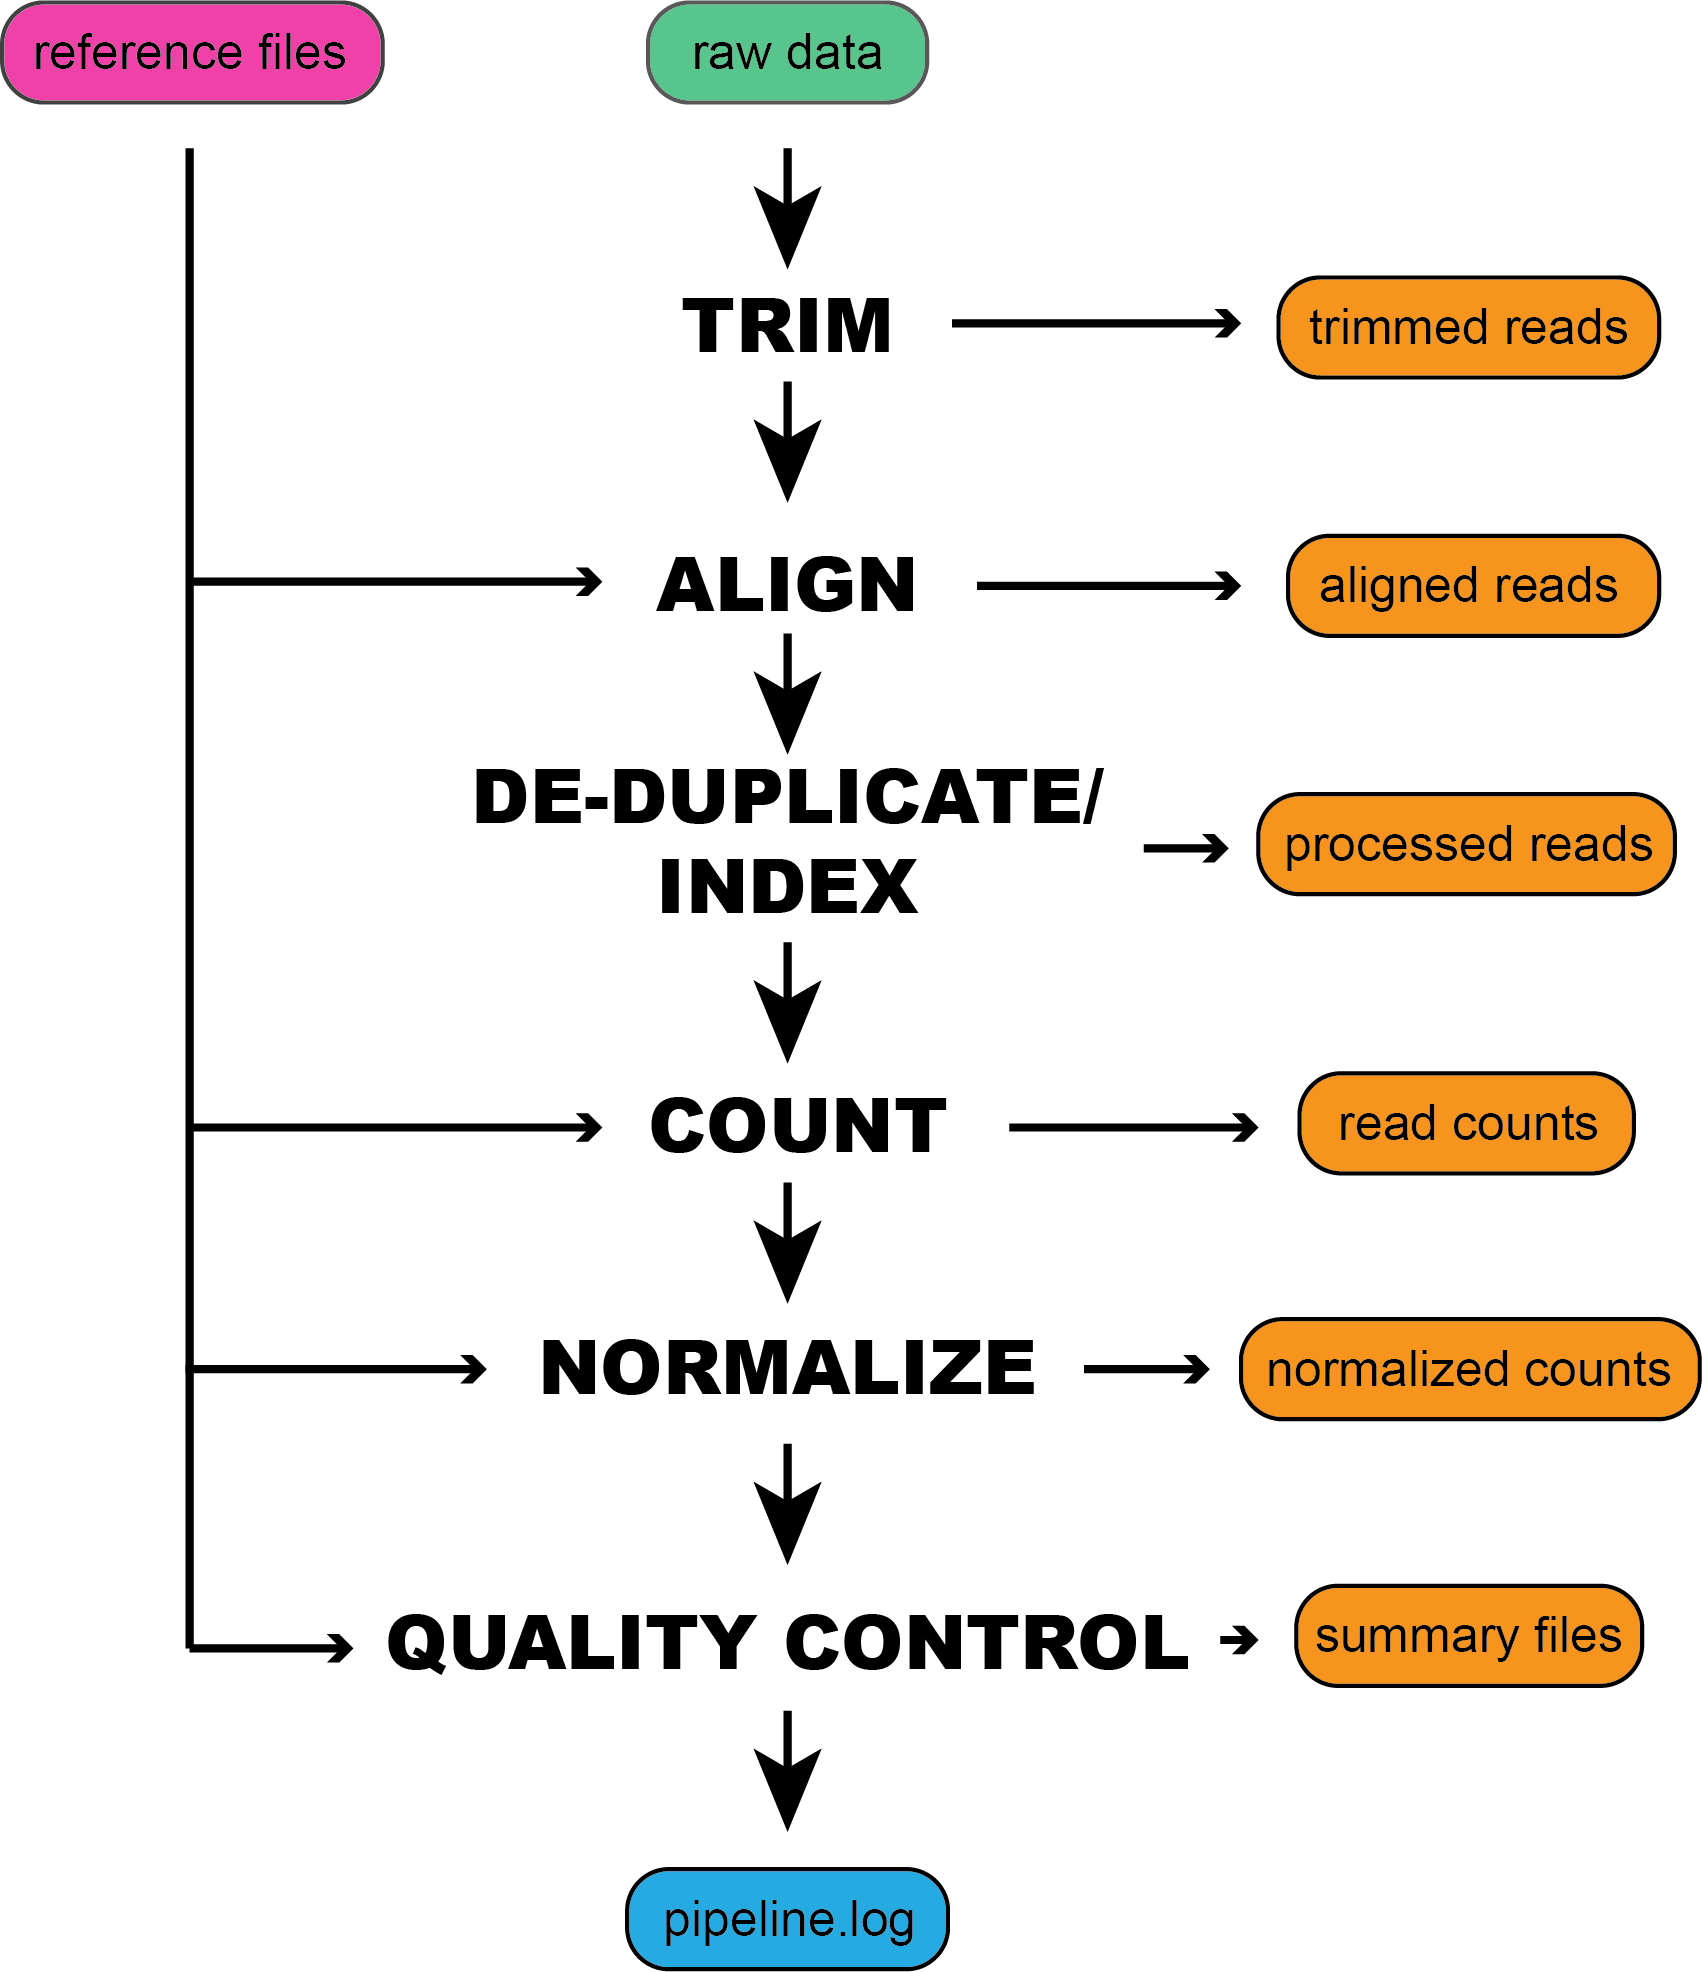
\includegraphics[width=120mm]{figures/xpresspipe_overview.png}
  \caption{An example schematic of the inputs required by XPRESSpipe and organization of the ouputs.}
  \label{fig:outputs}
\end{figure}


\subsubsection{Analyses}
XPRESSpipe has two analytical sub-modules. The first acts as a wrapper for the R package, DESeq2 \cite{deseq2}, to perform differential expression analysis on their data. More information on this sub-module can be found in the documentation (https://xpresspipe.readthedocs.io/en/latest/).

The second analytical tool introduced in XPRESSpipe is \texttt{rrnaProbe}. Ribosomal RNA (rRNA) contamination is common in RNA-seq library preparation and the bulk of RNA in a cell at any given time is dedicated to rRNA. As unique rRNA sequences are relatively few and therefore highly repeated in sequencing libraries without depletion. Depletion of these sequences is often desired in order to have better depth of coverage of mRNA sequences. In order to facilitate this depletion, many commercial kits are available that target specific rRNA sequences for depletion, or that enrich mRNA polyA tails. However, and especially in the case of ribosome profiling experiments, where RNA is digested by an RNase to create ribosome footprints, many commercial depletion kits will not perform sufficiently and polyA selection kits are inoperable as footprints will not have the requisite polyA sequence. To this end, custom rRNA probes are recommended \cite{ingolia_meth, ingolia_science}. \texttt{rrnaProbe} works on a directory containing fastqc \cite{fastqc} zip compressed files to detect over-represented sequences for each sample. These sequences are then collated to create consensus fragments. A rank ordered list of over-represented fragments within the appropriate length range to target for depletion is then output. A BLAST \cite{blast} search on consensus sequences intended for probe useage can then be performed to verify the fragment maps to an rRNA sequence and is thus a suitable depletion probe.

\subsection{XPRESStools}
XPRESStools is a python library of analysis features that builds upon existing packages, such as Matplotlib \cite{matplotlib} and Seaborn \cite{seaborn} to generate flexible, specific analyses and plots frequently used by biological researchers that can each be executed in a single line of code rather then tens to hundreds. Additionally, many included analytical features are currently available in an R package but not in a Python package, a programming language becoming more and more common in biological research. A summary of new or more automated tools is provided below and methods are discussed in subsequent sections. We refer the reader to the documentation (https://xpresstools.readthedocs.io/en/latest/?badge=latest) for more details instructions for other features currently in the toolkit, as well as for future features to be added.

\subsubsection{Getting Data}
XPRESStools is designed for analyzing gene expression data, but it is tractable to most data types assuming two conditions are met:

\begin{enumerate}
  \item \textbf{Expression Matrix}: It is assumed the input data matrix = \textit{i} * \textit{j} where \textit{i} (columns) are samples and \textit{j} (rows) are genes or other relative measurement points.
  \item \textbf{Metagene Table}: It is assumed the metagene table is a two column, header-less data matrix where column 0 is the sample ID (as specified in \textit{i} of the expression matrix) and column 1 is the sample group (for example, wild-type or treatment).
\end{enumerate}

Several functions are built into XPRESStools for importing and formatting this data. Options include importing microarray and RNAseq expression data and metadata from the GEO database, as well as custom data and metadata that follows required formatting requirements. Several methods for normalization, such as RPM, RPKM, FPKM, TPM and log-scale normalization are accessible within this toolkit.

\subsubsection{Analyzing Data}

While a litany of analysis tools are included in XPRESStools as of the time of writing, we will focus on tools unique to this Python library and refer to reader to the documentation for further details and examples of analysis features, current and future.

\begin{itemize}
  \item \textbf{Principle Components Analysis}: Principle components analysis (PCA) for the data matrix are performed with Python's scikit-learn package \cite{scikit_learn} and desired principle components are plotted in a scatter plot via the matplotlib \cite{matplotlib} and seaborn \cite{seaborn} packages. The XPRESStools PCA module, as in many other analysis modules within XPRESStools, samples are color-coded by cross-referencing the data matrix with the metagene table to determine sample label. A dictionary is additionally passed into the function that maps a particular color to each sample label. Confidence intervals are plotted over the scatterplot using numpy \cite{numpy1, numpy2} functionality as follows:

  \begin{enumerate}
    \item Compute the covariance of the two principle component arrays, \textit{x} and \textit{y} using the numpy.cov() function.

    \item Compute the eigenvalues and normalized eigenvectors of the covariance matrix using the numpy.linalg.eig() function.

    \item Compute the $\theta$ of the normalized eigenvectors using the numpy.arctan2() function and converting the output from radians to degrees using numpy.deg().

    \item Compute the $\lambda$ of the eigenvalues by taking the square root of the eigenvalues.

    \item Plot the confidence intervals over the scatter plot: The center point of the confidence interval is determined from the means of the \textit{x} and \textit{y} arrays. The angle is set equal to $\theta$. The width of the condfidence interval is calculated by
    \[
    \textit{w} = \lambda _{\textit{\scriptsize{x}}}\ \cdot\ \textit{ci}\ \cdot\ 2
    \]
    where \textit{ci} is equal to the corresponding confidence level (i.e. 68\% = 1, 95\% = 2, 99\% = 3). The heighth is similarly computed by
    \[
    \textit{h} = \lambda _{\textit{\scriptsize{y}}}\ \cdot\ \textit{ci}\ \cdot\ 2
    \]
  \end{enumerate}

  \item \textbf{Volcano Plot}: Volcano plots are an efficient method for plotting magnitude, direction, and significance of changes in expression or other data types between two conditions with multiple replicates each. By providing the categorical names for samples of two conditions in the metadata matrix, XPRESStools will automate the calculation and plotting of this plotting method. For each gene, expression levels are averaged between the two conditions and the log\textsubscript{2}(fold change) is calculated. Additionally, for each gene, the P-value between the two conditions is calculated using scipy's individual T-test function \cite{scipy}. The log\textsubscript{2}(fold change) and -log\textsubscript{10}(P-value) is then plotted for each gene between the two conditions. Additional features available are the ability to plot threshold lines, highlight subsets of genes within the plot, and label specific genes by name.

\end{itemize}

\subsection{Availability}
The source code for these packages is open source and protected under the GPL-3.0 license. The code can be publicly accessed and installed from https://github.com/XPRESSyourself. Updates to the software are version controlled and maintained on GitHub. XPRESStools is pip installable. XPRESSpipe is available as a Docker image. Jupyter notebooks and video walkthroughs are included on https://github.com/XPRESSyourself for guiding a user through use of the packages. Documentation is hosted on readthedocs \cite{readthedocs}.

\subsection{Cost Analysis}
Perform an example run using Docker image on AWS and give a cost per sample and time per sample output.


\section{Results and Discussion}

\subsection{Validation}
In order to evaluate the ability of XPRESSpipe to provide the user with reliable results, we processed publicly available raw sequence files through the pipeline. We chose to highlight a ribosome profiling dataset and a subset of TCGA samples.

\subsubsection{Ribosome Profiling Dataset}
In this section, we will look at the count values available on GEO and the counts we get out of the pipeline. Fig 2A will be correlations showing tight relationships between all mapped genes. F2B-D will replicate the relevant figures from the paper.

\subsubsection{TCGA Dataset}
In this section, we will process the raw data for 10-20 TCGA samples and compare the FPKM counts output by XPRESSpipe to the publicly available FPKM counts for the relevant samples.

\subsubsection{Ease of Use Case Study}
In this section, we will discuss a simple case study of 2-4 users with no computational experience and the time it took to get output and the quality of the output.

\subsection{New Insights into Metabolism}
Using the previously discussed ribosome profiling dataset, we will discuss new metabolic insights obtained by focusing on something other than what the authors were interested in. THe way this is explained will be fairly important -- do we want to highlight that this is capable of finding something new (I don't know that that is really the purpose of this), that this just makes it so someone can quickly access the data and re-analyze it for their points of interest? Highlight again the amount of sequencing data out there and how most have only be used to explore one narrow aspect of biology. Figure 3 will include the insights gained. A potential Fig4 discussing validation of the insights.


\section{Conclusions}
We have described herein a new software suite, XPRESSyourself, a collection of tools and pipelines to aid in expression data processing and analysis. The software was designed to be flexible and modular so that in the future, new modules and tools can be easily added to and tested in the software suite.
Discuss results of validation and biological study


\section*{Acknowledgments}
J.A.B. received support from the National Institute of Diabetes and Digestive and Kidney Diseases (NIDDK) Inter-disciplinary Training Grant T32 Program in Computational Approaches to Diabetes and Metabolism Research, 1T32DK11096601 to Wendy W. Chapman and Simon J. Fisher.


\section*{Contributions}
\begin{tabular}{ l l }
 Conceptualization & J.A.B. \\
 \hline
 Supervision & M.T.H., J.G., A.R.Q., J.P.R. \\
 \hline
 Project Administration & J.A.B. \\
 \hline
 Investigation & J.A.B. \\
 \hline
 Formal Analysis & J.A.B. \\
 \hline
 Software & J.A.B., J.R.B. \\
 \hline
 Methodology & J.A.B., J.R.B., M.T.H. \\
 \hline
 Validation & J.A.B., J.T.M., A.J.B., Y.O. \\
 \hline
 Resources & J.A.B., J.P.R. \\
 \hline
 Funding Acquisition & J.A.B., J.P.R. \\
 \hline
 Writing - Original Draft & J.A.B. \\
 \hline
 Writing - Review \& Editing & J.A.B., M.T.H., J.G., A.R.Q., J.P.R. \\
 \hline
 Visualization & J.A.B.
\end{tabular}


\bibliography{manubib}
\bibliographystyle{Science}

\end{document}
